\documentclass{article}
\usepackage[UTF8]{ctex}
\usepackage{amsmath,mathtools,geometry,pgfplots,float,mathrsfs,caption,enumerate}
\pgfplotsset{compat=1.15}
\usetikzlibrary{arrows}
\geometry{scale=0.7}

\title{每日一题(19.2)}
\author{\kaishu 李政毅}
\date{2022年6月1日}

\begin{document}
\maketitle
\begin{enumerate}
	\renewcommand{\labelenumi}{\textbf{\theenumi. }}
	\item 如图, $P$为正$\triangle ABC$内一点, 且$PA=3$, $PB=4$, $PC=5$, 求$\angle APB$.
	\begin{figure}[H]
		\flushright
		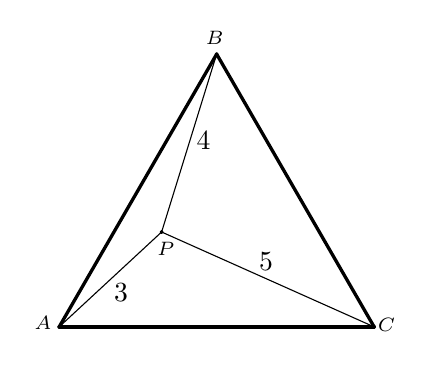
\begin{tikzpicture}[line cap=round,line join=round,>=triangle 45,x=1.0cm,y=1.0cm]
			\clip(-0.4,-0.2) rectangle (4.4,3.8);
			\draw [line width=0.4pt] (2.,3.4641016151377544)-- (1.3010751819210529,1.2051410923961794);
			\draw [line width=0.4pt] (1.3010751819210529,1.2051410923961794)-- (0.,0.);
			\draw [line width=0.4pt] (1.3010751819210529,1.2051410923961794)-- (4.,0.);
			\draw [line width=1.2pt] (2.,3.4641016151377544)-- (0.,0.);
			\draw [line width=1.2pt] (0.,0.)-- (4.,0.);
			\draw [line width=1.2pt] (4.,0.)-- (2.,3.4641016151377544);
			\draw (0.5748727123502351,0.6698878182589716) node[anchor=north west] {$3$};
			\draw (2.4139488310797336,1.0729404237241665) node[anchor=north west] {$5$};
			\draw (1.6205175304982108,2.6045372192330645) node[anchor=north west] {$4$};
			\begin{scriptsize}
				\draw [fill=black] (2.,3.4641016151377544) circle (0.5pt);
				\draw[color=black] (1.9757836163786457,3.672165627637209) node {$B$};
				\draw [fill=black] (0.,0.) circle (0.5pt);
				\draw[color=black] (-0.20558111750870883,0.046226244330159046) node {$A$};
				\draw [fill=black] (4.,0.) circle (0.5pt);
				\draw[color=black] (4.1571483502660005,0.023020232276993922) node {$C$};
				\draw [fill=black] (1.3010751819210529,1.2051410923961794) circle (0.5pt);
				\draw[color=black] (1.3550229075330422,0.9846952837092982) node {$P$};
			\end{scriptsize}
		\end{tikzpicture}
	\end{figure}
	\item 如图, $P$为外$\triangle ABC$内一点, 且$PA=3$, $PB=4$, $PC=5$, 求$\angle APB$.
	\begin{figure}[H]
		\flushright
		\definecolor{uuuuuu}{rgb}{0.26666666666666666,0.26666666666666666,0.26666666666666666}
		\begin{tikzpicture}[line cap=round,line join=round,>=triangle 45,x=1.0cm,y=1.0cm]
			\clip(-6.,-0.5) rectangle (4.6,4.);
			\draw [line width=1.2pt] (2.,3.4641016151377544)-- (0.,0.);
			\draw [line width=1.2pt] (0.,0.)-- (4.,0.);
			\draw [line width=1.2pt] (4.,0.)-- (2.,3.4641016151377544);
			\draw (-3.1882031643676894,0.874452316813536) node[anchor=north west] {$3$};
			\draw (-0.12921245839102044,1.1901489243016161) node[anchor=north west] {$5$};
			\draw (-1.8927587016942957,3.073442479316715) node[anchor=north west] {$4$};
			\draw [line width=0.4pt] (-5.591230622502539,1.7025504191743688)-- (2.,3.4641016151377544);
			\draw [line width=0.4pt] (-5.591230622502539,1.7025504191743688)-- (0.,0.);
			\draw [line width=0.4pt] (-5.591230622502539,1.7025504191743688)-- (4.,0.);
			\begin{scriptsize}
				\draw [fill=black] (2.,3.4641016151377544) circle (0.5pt);
				\draw[color=black] (1.9609164225610096,3.851797908123533) node {$B$};
				\draw [fill=black] (0.,0.) circle (0.5pt);
				\draw[color=black] (-0.3142759530586481,-0.28491625896165496) node {$A$};
				\draw [fill=black] (4.,0.) circle (0.5pt);
				\draw[color=black] (4.290539237788793,0.041666438439807295) node {$C$};
				\draw [fill=uuuuuu] (-5.591230622502539,1.7025504191743688) circle (0.5pt);
				\draw[color=uuuuuu] (-5.800864265557727,1.9685043531084345) node {$P$};
			\end{scriptsize}
		\end{tikzpicture}
	\end{figure}
\end{enumerate}
\end{document}